\section{Application Architecture}\label{sec:applicationArchitecture}

The main objective of this work is to create a generic platform for Supply Chain Management (SCM). \ac{SCM-BP} is divided into four main modules described below: WebApp - frontend, WebApp - backend, Blockchain network and Data Storage. Figure~\ref{fig:detalhamentotecnico} shows the application architecture and its components. Figure~\ref{fig:dataStructure} present the main data structure.

\begin{figure}[htbp]
\begin{center}
  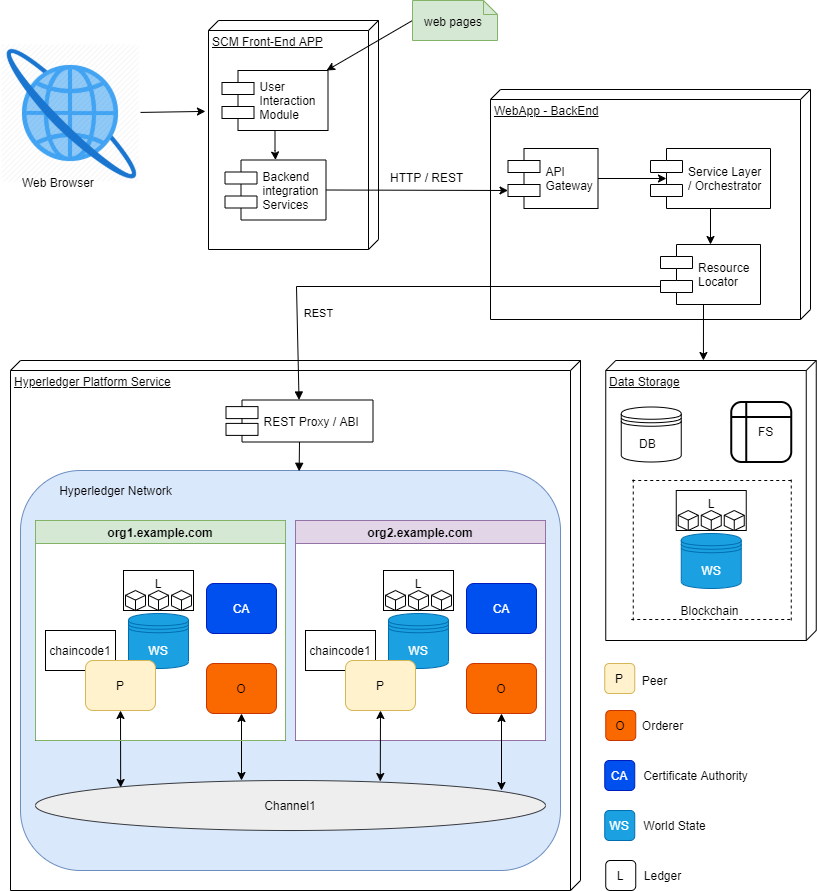
\includegraphics[scale=0.55]{images/architecture.png}
\caption{Application architecture of \ac{SCM-BP}}
\label{fig:detalhamentotecnico}
\end{center}
\end{figure}

In the table~\ref{table:userStories} are defined the main functional requirements in order to be able to meet all the objectives proposed by this project. Are characterized as non-functional requirements for the proper functioning the items in table~\ref{table:rnf}.



\subsection{WebApp - FrondEnd}\label{sec:WebAppFrondEnd}
WebApp - FrontEnd is a client–server computer application which the client (including the user interface and client-side logic) runs in a web browser. This is a single-page application (SPA), a web application that interacts with the user by dynamically rewriting the current page rather than loading entire new pages from a server. This approach avoids interruption of the user experience between successive pages, making the application behave more like a desktop application.

The application is build with React (also known as React.js or ReactJS). This is a JavaScript library for building user interfaces. It is maintained by Facebook and a community of individual developers and companies. Used as a base in the development of single-page or mobile applications, React is optimal for fetching rapidly changing data that needs to be recorded. However, fetching data is only the beginning of what happens on a web page, which is why complex React applications usually require the use of additional libraries for state management, routing, and interaction with an API.

The Webapp - FrontEnd is divided into two main blocks and these are classified according to the interactions: User Interaction Modules and Backend Interactions Services.

\subsubsection{User Interaction}\label{sec:UserInteraction}
The User Interaction modules are responsible for providing web pages that will be rendered on client’s web browser. These interactions are provided by web pages grouped by the following modules:

\begin{itemize}
\item Login page
\item Application configuration module
\item User handling module (actors - CRUD)
\item Data entry module (forms)
\item Data visualization module
\item Reporting module
\end{itemize}

\subsubsubsection{Login Module}
The Login Module is responsible for display the login and authentication alternatives pages (‘forgot my password’, ‘reset my password’, etc.).

\subsubsubsection{Application configuration module}
The Application configuration module provides the features of creation/configuration of supply chain items and supply chain flows (steps and sub-tasks).

\subsubsubsection{User handling module}
This module provides the features for creation/configuration of Actors and Roles. The table in appendix \ref{app:userCreationFields} show the fields and values for creating a user.

\subsubsubsection{Data entry module}
The Data entry module provides form pages that allow users to enter data in the application, search and move assets from a step to another.

\subsubsubsection{Data visualization module}
The Data visualization module is responsible to display the information about assets in the supply chain flow. 

\subsubsubsection{Reporting Module}
In the Reporting module users can generate reports/files containing information organized in a narrative, graphic, or tabular form, prepared on ad hoc, periodic, recurring, regular, or as required basis. Reports may refer to specific periods, events, occurrences, or subjects, and may be presented in written form or any other format.

\subsubsection{Backend Interaction}\label{sec:BackendInteraction}
Backend interactions happen via a service layer consisting of:

\begin{itemize}
\item Authentication service
\item Application setup service
\item User creation service (actors)
\item Data entry service (forms)
\item Data visualization service
\item Reporting service
\end{itemize}

\subsubsubsection{Authentication Service}
The function of the Authentication Service is to request information from an authenticating party, and validate it against the configured identity repository using the specified authentication module. After successful authentication, the user session is activated and can be validated across all web applications participating in an SSO environment. For example, when a user or application attempts to access a protected resource, credentials are requested by one (or more) authentication modules. Gaining access to the resource requires that the user or application be allowed based on the submitted credentials.

\subsubsubsection{Application setup Service}
Application setup service provides methods to configure and edit  supply chain items and supply chain flows, defining which steps and sub-tasks will be present in this flow and which information will be present in these steps.

\subsubsubsection{User creation Service}
This service is responsible for the creation of users and roles, to allow them to log in and use the application’s features. Only Administrators are allowed to create new users (see Actions and Actors).

\subsubsubsection{Data entry Service}
Data entry service receives data from UI forms and send them to the backend to be processed and stored.

\subsubsubsection{Data visualization Service}
Data visualization services provides information about the supply chain: Assets, users and transactions, to be used by the data visualization module.

\subsubsubsection{Reporting Service}
Report services generate files (Doc/PDF/XSL, etc...) from a specific period of time with information about the supply chain: Assets, users and transactions.
\subsection{WebApp - BackEnd}\label{sec:WebAppBackEnd}
WebApp - BackEnd is a Middleware that runs on the server. This Middleware (server-side software) facilitates client-server connectivity, forming a middle layer between the app(s) and the network: the server, the database, the operating system, and more. It receives requests from the clients (in this case, the WebApp - FrontEnd), and contains the logic to send the appropriate data back to the applicant, over HTTP and REST.  These are the main conventions that provide structure to the request-response cycle between clients and servers.

WebApp - BackEnd is an application build with Node.js, an application platform where developers can write Javascript programs that are compiled, optimized and interpreted by the V8 virtual machine. Node.js can create quick, reliable websites and products in much efficient manner. Developing easy to scale real time applications in other technologies is bit difficult, but JavaScript technologies made it easier.

The WebApp - BackEnd is composed by the API Gateway, Service Layer and Resource Locator more detailed below.

\subsubsection{API Gateway}\label{sec:APIGateway}
API Gateway is a managed service that enables easily create, publish, maintain, monitor and secure REST APIs to act as a "gateway" for applications to access data, business logic, or functionality in the backend services, such as workloads. The API Gateway provides a simple uniform view of external resources to the internals of this application. It manages all tasks involved in receiving and processing API calls, including traffic management, authorization and access control, monitoring and management of API versions.

\begin{figure}[htbp]
\begin{center}
  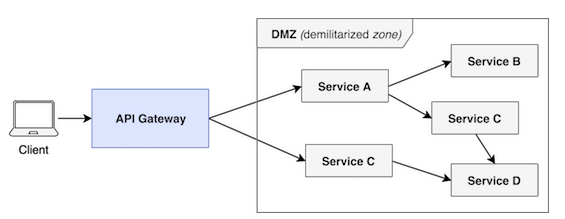
\includegraphics[scale=0.75]{images/apigateway.png}
\caption{API Gateway.}
\label{default-regular2}
\end{center}
\end{figure}

Basically, the Gateway is an interface that receives calls to its internal systems, being a large gateway. It act in five different ways:

\begin{itemize}
\item Filter for call traffic from different media;
\item Single gateway to the various APIs that are exposed;
\item Router: API and Rate Limit traffic router;
\item Security engine with authentication and logging.
\end{itemize}

Gateway access can be done from many different devices. Therefore, it must have the power to unify outgoing calls and be able to deliver to the user content that can be accessed from any browser and system. In this project the gateway interaction happens with the frontend webapp. The Gateways as a Security Feature: In the APIs world, one of the most subject talked about issues is always security, and having an API Gateway is one of the best solutions on the market to get full control of API’s, because this pattern addresses the so-called CIA (Confidentiality, Integrity, Availability) almost flawlessly.

\subsubsection{Service Layer}\label{sec:ServiceLayer}
A Service Layer defines an application's boundary and its set of available operations from the perspective of interfacing client layers. It encapsulates the application's business logic, controlling transactions and coordinating responses in the implementation of its operations.

Enterprise applications typically require different kinds of interfaces to the data they store and the logic they implement: data loaders, user interfaces, integration gateways, and others. Despite their different purposes, these interfaces often need common interactions with the application to access and manipulate its data and invoke its business logic. The interactions may be complex, involving transactions across multiple resources and the coordination of several responses to an action. Encoding the logic of the interactions separately in each interface causes a lot of duplication. the service layer provides:

\begin{enumerate}
\item Centralizes external access to data and functions.
\item Hides (abstracts) internal implementation and changes.
\item Allows for versioning of the services.
\end{enumerate}

The service layer acts as an orchestrator, controlling the flow of incoming and outcoming information requests and responses. Orchestration allows to directly link process logic to service interaction within workflow logic. This combines business process modeling with service-oriented modeling and design, realizing workflow management through a process service model. Orchestration brings the business process into the service layer, positioning it as a master composition controller.

\subsubsection{Resource Locator}\label{sec:ResourceLocator}

Resource locators are components that abstracts the persistence layer. Their job is to provide an object that can help services to discover and persist information from/to the Data Storage Module. Information can be stored in the Blockchain, Filesystem or Database and resource locators should know exactly where get/put data within them.  
\subsection{Blockchain}\label{sec:BlockchainModule}

SCM-BP uses blockchain as a supply chain that tracks parts and service provenance, ensures the authenticity of goods, blocks counterfeits, and reduces conflicts. In SCM- BP, the Blockchain module consists of a smart contract, chaincode, and ledger. From the application developer's perspective, a smart contract and the ledger form the heart of a Hyperledger Fabric blockchain system. Whereas a ledger holds facts about the current and historical state of a set of business objects, a smart contract defines the executable logic that generates new facts added to the ledger. 
Based on the discussion in section \ref{sec:versus} and to achieve the non-functional requirements exposed in appendix \ref{app:Non-functional}, the permissioned blockchain was chosen and Hyperledger Fabric as its implementation. 

\subsubsection{Smart contract}
Before businesses can transact with each other, they must define a common set of contracts covering common terms, data, rules, concept definitions, and processes. Together, these contracts lay out the business model that governs all of the interactions between transacting parties.

A smart contract defines the rules between different organizations in executable code. Applications invoke a smart contract to generate transactions that are recorded on the ledger.

\subsubsection{Chaincode}
Hyperledger Fabric users often use the terms smart contract and chaincode interchangeably. In general, a smart contract defines the transaction logic that controls the lifecycle of a business object contained in the world state. It is then packaged into a chaincode which is then deployed to a blockchain network. Think of smart contracts as governing transactions, whereas chaincode governs how smart contracts are packaged for deployment.

\subsubsection{Ledger}
At the simplest level, a blockchain immutably records transactions that update states in a ledger. A smart contract programmatically accesses two distinct pieces of the ledger: a blockchain, which immutably records the history of all transactions and a world state that holds a cache of the current value of these states, as it’s the current value of an object that is usually required.

The ledger is the sequenced, tamper-resistant record of all state transitions in the fabric. State transitions are a result of chaincode invocations (‘transactions’) submitted by participating parties. Each transaction results in a set of asset key-value pairs committed to the ledger as creates, updates, or deletes. The ledger comprises a blockchain (‘chain’) to store the immutable, sequenced record in blocks, as well as a state database to maintain the current fabric state. There is one ledger per channel. Each peer maintains a copy of the ledger for each channel of which they are a member.

Smart contracts primarily put, get, and delete states in the world state and query the immutable blockchain record of transactions.

\begin{itemize}
\item A \textbf{get} typically represents a query to retrieve information about the current state of a business object.
\item A \textbf{put} typically creates a new business object or modifies an existing one in the ledger world state.
\item A \textbf{delete} typically represents the removal of a business object from the current state of the ledger but not its history.
\end{itemize}

Smart contracts have many APIs available to them. Critically, in all cases, whether transactions create, read, update or delete business objects in the world state, the blockchain contains an immutable record of these changes.


\subsection{Data Storage}\label{sec:DataStorage}
Data storage is a general term for archiving data in electromagnetic or other forms for use by a computer or device. Different types of data storage play different roles in a computing environment. In addition to forms of hard data storage, there are now new options for remote data storage, such as cloud computing and blockchain, that can revolutionize how users save and access data.  

SCM-BP uses three applications as data storage: Blockchain, Cloud filesystem, and relational database, which are better detailed in the following subsections. Blockchains grow continuously because of the amount of data and code in them, which is unchanging. Therefore, an important design decision is to choose which data and calculations to keep in and out of the chain.

\subsubsection{Filesystem}\label{sec:Filesystem}
A cloud file system is a tiered storage system that provides shared access to file data. Users can create, delete, modify, read and write files and logically organize them into directory trees for intuitive access.

Cloud file-sharing can be defined as a service that gives multiple users simultaneous access to a cloud file data set. Cloud file sharing security is managed with the user and group permissions, allowing administrators to control access to shared file data tightly.

For all files uploaded and stored in the filesystem, a locally stored digital fingerprint (hash) is saved in the blockchain, separately from the original files or content, to make it easier to confirm whether data has been altered or manipulated in a particular organization.

\subsubsection{Database}\label{sec:Database}
A relational database is a set of formally described tables from which data can be accessed or reassembled in many different ways without reorganizing the database tables. The standard user and \ac{API} of a relational database is the \ac{SQL}. SQL statements are used for interactive queries for information from a relational database and for gathering data for reports.

\subsubsection{Blockchain}\label{sec:DataStorageBlockchain}

Since the blockchain consists of a Ledger and a world state database (among other components), this can also be seen as part of the data storage module as it stores data. Component \ref{sec:ResourceLocator} has the intelligence to decide where to search and store data to optimize storage consumption.